V tem podpoglavju bodo predstavljene različne metode izgradnje priponskih dreves. Metode bodo predstavljene v zaporedju od najbolj počasne, ki izgradi priponsko drevo v času $O(n^3)$, do najhitrejše, ki izgradi drevo v času $O(n)$. 

\paragraph{Naivna metoda:}
Ta metoda v vsakem koraku s sprehodom po drevesu podaljša vse pripone za en znak ter doda novo pripono. Metoda v $i$-tem koraku izgradnje v dosedaj izgrajeno drevo, ki je bilo izgrajeno za podniz $T[1,i-1]$, doda znak $T[i]$ ter tako izgradi drevo za podniz $T[1,i]$. To je storjeno z dodajanjem pripone, ki predstavlja znak $T[i]$, in s podaljševanjem pripon, ki že obstajajo v drevesu. Ker listi vedno predstavljajo konec pripone, se niz na povezavi, ki vodi v list, podaljša za en znak.

\begin{figure}[htb]
    \begin{subfigure}[t]{0.3\linewidth}
        \subcaption*{}
            \includesvg{Slike/Naivna/KOKOŠNaivnaK.svg}
            \centering
            \label{fig:Naivna1}
        \end{subfigure}
        \hspace{0.5cm}
        \begin{subfigure}[t]{0.3\linewidth}
            \subcaption*{}
            \includesvg{Slike/Naivna/KOKOŠNaivnaOKOŠ.svg}
            \centering
            \label{fig:Naivna2}
        \end{subfigure}
        \hspace{0.5cm}
        \begin{subfigure}[t]{0.3\linewidth}
            \subcaption*{}
            \includesvg{Slike/Naivna/KOKOŠNaivnaKOŠ.svg}
            \centering
            \label{fig:Naivna3}
        \end{subfigure}
        
        \begin{subfigure}[t]{0.3\linewidth}
            \subcaption*{}
            \includesvg{Slike/Naivna/KOKOŠNaivnaOŠ.svg}
            \centering
            \label{fig:Naivna4}
        \end{subfigure}
        \hspace{0.5cm}
        \begin{subfigure}[t]{0.3\linewidth}
            \subcaption*{}
            \includesvg[scale=0.67]{Slike/Naivna/KOKOŠNaivnaŠ.svg}
            \centering
            \label{fig:Naivna5}
        \end{subfigure}
        \hspace{0.5cm}
        \begin{subfigure}[t]{0.3\textwidth}
            \subcaption*{}
            \includesvg[scale=0.67]{Slike/Naivna/KOKOŠNaivnaS.svg}
            \centering
            \label{fig:Naivna6}
    \end{subfigure}

    %   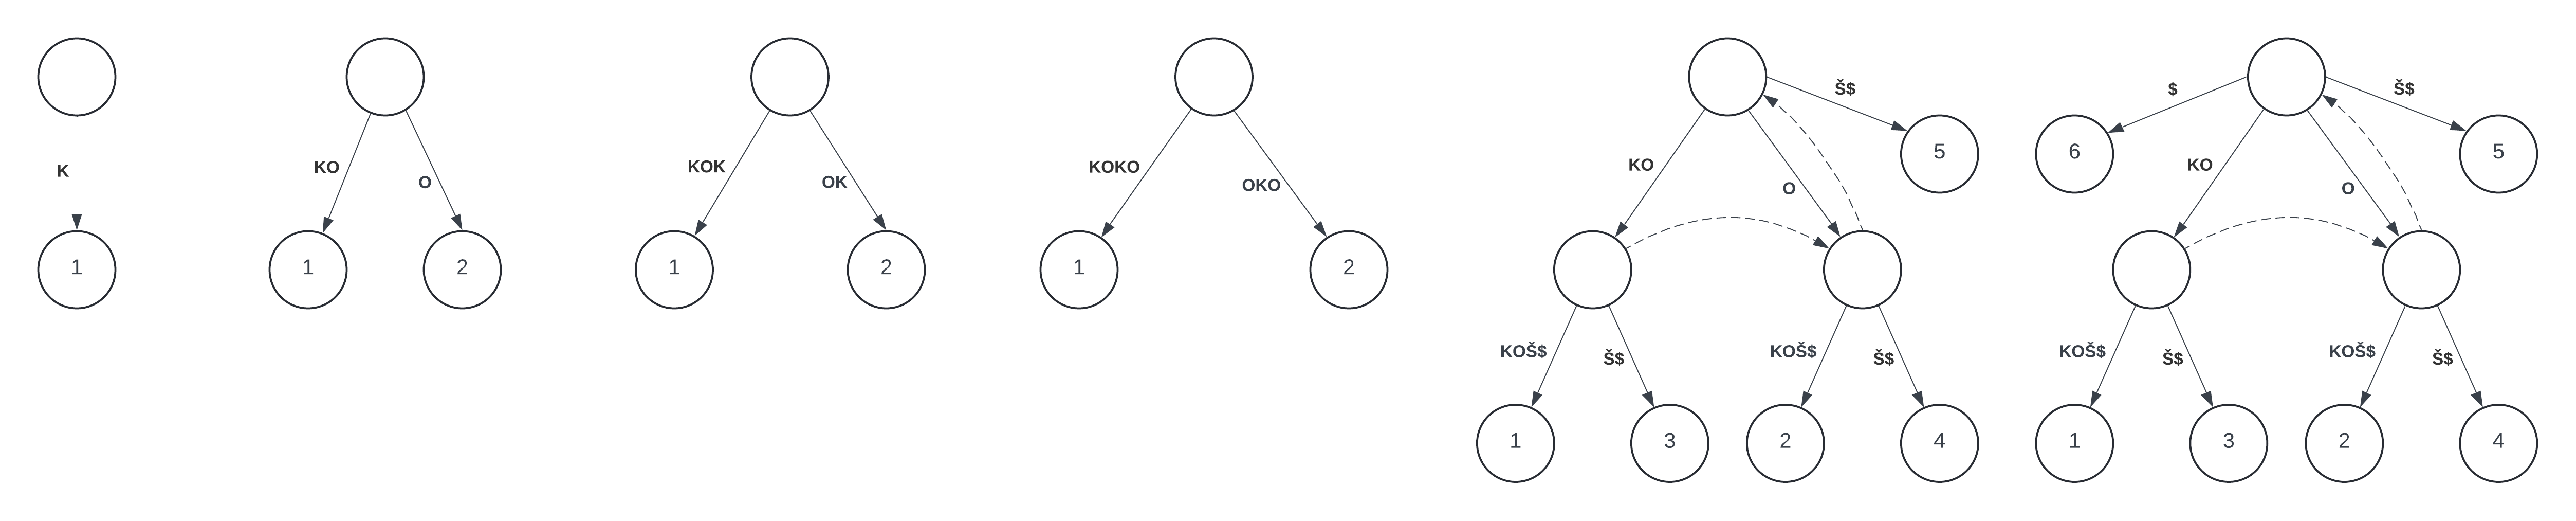
\includegraphics[width=\textwidth]{Slike/KOKOSUkkonen.png}
    \caption{Primer izgradnje priponskega drevesa z uporabo Naivne metode za besedo »KOKOŠ$\$$«.} 
    \label{fig:Naivna}
\end{figure}

Opazimo, da drevo, ki  je zgrajeno za podniz T[1,i], $i< n$, ni nujno priponsko, saj niso vse pripone podniza T[1,i] shranjene v listih. Še več, nekatere pripone niso niti eksplicitno predstavljene. Kljub temu pa to drevo vsebuje vso informacijo o pripadajočlh priponah, pri čemer moramo posebej beležiti vse implicitno predstavljene pripone. Takšnemu drevesu rečemo implicitno priponsko drevo. Ta problem se reši z beleženjem takih pripon. Če se niz na povezavi, ki predstavlja zadnji del implicitne pripone, nadaljuje po priponi z znakom $T[i]$ se ne stori ničesar, saj je tudi podalšana pripona implicitno predstavljena. Če pa se niz na povezavi, ki predstavlja zadnji del implicitne pripone, ne nadaljuje z znakom $T[i]$, pa se povezavo razdeli na dva dela in se ustavri vozlišče, na katerega kaze povezava z nizom, ki se ujema z predhodnjo pripono, ter ima dva otroka: vozlišče na katerega kaže prostanek predhodnje povezave ter list z znakom $T[i]$. V primeru, da vozlišče že obstaja, se le temu doda novega otroka, na katerega kaže povezava z znakom, ki se razlikuje. Postopek izgradnje priponskega drevesa za besedo »KOKOŠ« z naivno metodo izgradnje je prikazan na Sliki \ref{fig:Naivna}. Na Sliki \ref{fig:Naivna} zgolj tretje (zadnje drevo v prvi vrstici) in četrto (prvo drevo v drugi vrstici) drevo sta implicitna priponska drevesa.

\begin{izr}\label{izr:naivna}
    Naivna metoda zgradi priponsko drevo nad besedo $T$, dolžine $n$, v času $O(n^3)$.
\end{izr}

\begin{proof}
    Naivna metoda se v vsakem koraku sprehodi čez celotno drevo. Črkovna globina vsakega vozlišča je največ dolžina že dodanega besedila v drevesu, v $i$-tem koraku je črkovna globina $\textit{Sd}(v)$ vsakega vozlišča $v$ je največ $i$. Podobno velja tudi za število listov v drevesu, ki ne presega dolžine že dodanega podniza. Globina lista je manjša ali enaka črkovni globini, torej velja, da se v $i$-tem koraku pregleda $\sum_{j=1}^i j=\dfrac{i(i+1)}{2}$ vozlišč.

    Ker je niz $T$ dolg $n$ znakov, je skozi celotno izgradnjo priponskega drevesa število obiskanih vozlišč enako
    $$
        \sum_{i=1}^n \sum_{j=1}^i j=\sum_{i=1}^n \dfrac{i(i+1)}{2}=\dfrac{n(n+1)(n+2)}{6}=O(n^3).
    $$
    Torej naivna metoda potrebuje $O(n^3)$ časa.
\end{proof}

\paragraph{Izboljšana naivna metoda:}
Naivna metoda je preprosti način izgradnje priponskega drevesa, vendar se hitro opazijo načini za pospešitev izgradnje drevesa. Najprej opazimo, da metoda nepotrebno pregleduje celotno drevo. To se lahko reši z uporabo priponskih povezav (angl. \textit{Suffix link}).

\begin{defi}\label{def:sl}
    Naj notranje vozlišče $v$ predstavlja niz $x\alpha$, kjer $x$ je znak in $\alpha\in\Sigma^*$ je podniz niza $T$. Priponska povezava $\textit{sl}(v)$ je povezava na notranje vozlišče $w$, ki predstavlja niz $\alpha$.

    %Priponska povezava $\textit{sl}(v)$ je povezava iz notranjega vozlišča $v$ v notranje vozlišče $w$. Vozlišče $v$ predstavlja niz $y=x\alpha $, medtem ko vozlišče $w$ pa predstavlja niz $\alpha\in\Sigma^*$. Pri tem je $x\in\Sigma$ znak.
\end{defi}

Na Sliki \ref{fig:PriponskoDrevo} sta priponski povezavi prikazani s črtkano puščico. Uvedba priponskih povezav omogoča izogib nepotrebnim sprehodom po drevesu. Tako metoda podaljša vse liste zgolj s sprehodom po priponskih povezavah. Pri tem se opazi, da metoda lahko beleži notranje vozlišče s povezavo na list, ki predstavlja najdaljšo pripono v predhodnjem koraku izgradnje $T[1,i-1]$. Beleženje tega vozlišča, ki ga imenujemo začetna točka, odstrani nepotrebno iskanje začetka sprehoda po priponskih povezavah.

\begin{figure}[htb]
    \begin{subfigure}[t]{0.3\linewidth}
        \subcaption*{}
        \includesvg{Slike/IzbolšanaNaivna/KOKOŠIzbolšanaNaivnaK.svg}
        \centering
        \label{fig:IzbolšanaNaivna1}
    \end{subfigure}
    \hspace{0.5cm}
    \begin{subfigure}[t]{0.3\linewidth}
        \subcaption*{}
        \includesvg{Slike/IzbolšanaNaivna/KOKOŠIzbolšanaNaivnaOKOŠ.svg}
        \centering
        \label{fig:IzbolšanaNaivna2}
    \end{subfigure}
    \hspace{0.5cm}
    \begin{subfigure}[t]{0.3\linewidth}
        \subcaption*{}
        \includesvg{Slike/IzbolšanaNaivna/KOKOŠIzbolšanaNaivnaKOŠ.svg}
        \centering
        \label{fig:IzbolšanaNaivna3}
    \end{subfigure}
    
    \begin{subfigure}[t]{0.3\linewidth}
        \subcaption*{}
        \includesvg{Slike/IzbolšanaNaivna/KOKOŠIzbolšanaNaivnaOŠ.svg}
        \centering
        \label{fig:IzbolšanaNaivna4}
    \end{subfigure}
    \hspace{0.5cm}
    \begin{subfigure}[t]{0.3\linewidth}
        \subcaption*{}
        \includesvg[scale=0.67]{Slike/IzbolšanaNaivna/KOKOŠIzbolšanaNaivnaŠ.svg}
        \centering
        \label{fig:IzbolšanaNaivna5}
    \end{subfigure}
    \hspace{0.5cm}
    \begin{subfigure}[t]{0.3\textwidth}
        \subcaption*{}
        \includesvg[scale=0.67]{Slike/IzbolšanaNaivna/KOKOŠIzbolšanaNaivnaS.svg}
        \centering
        \label{fig:IzbolšanaNaivna6}
    \end{subfigure}

    %   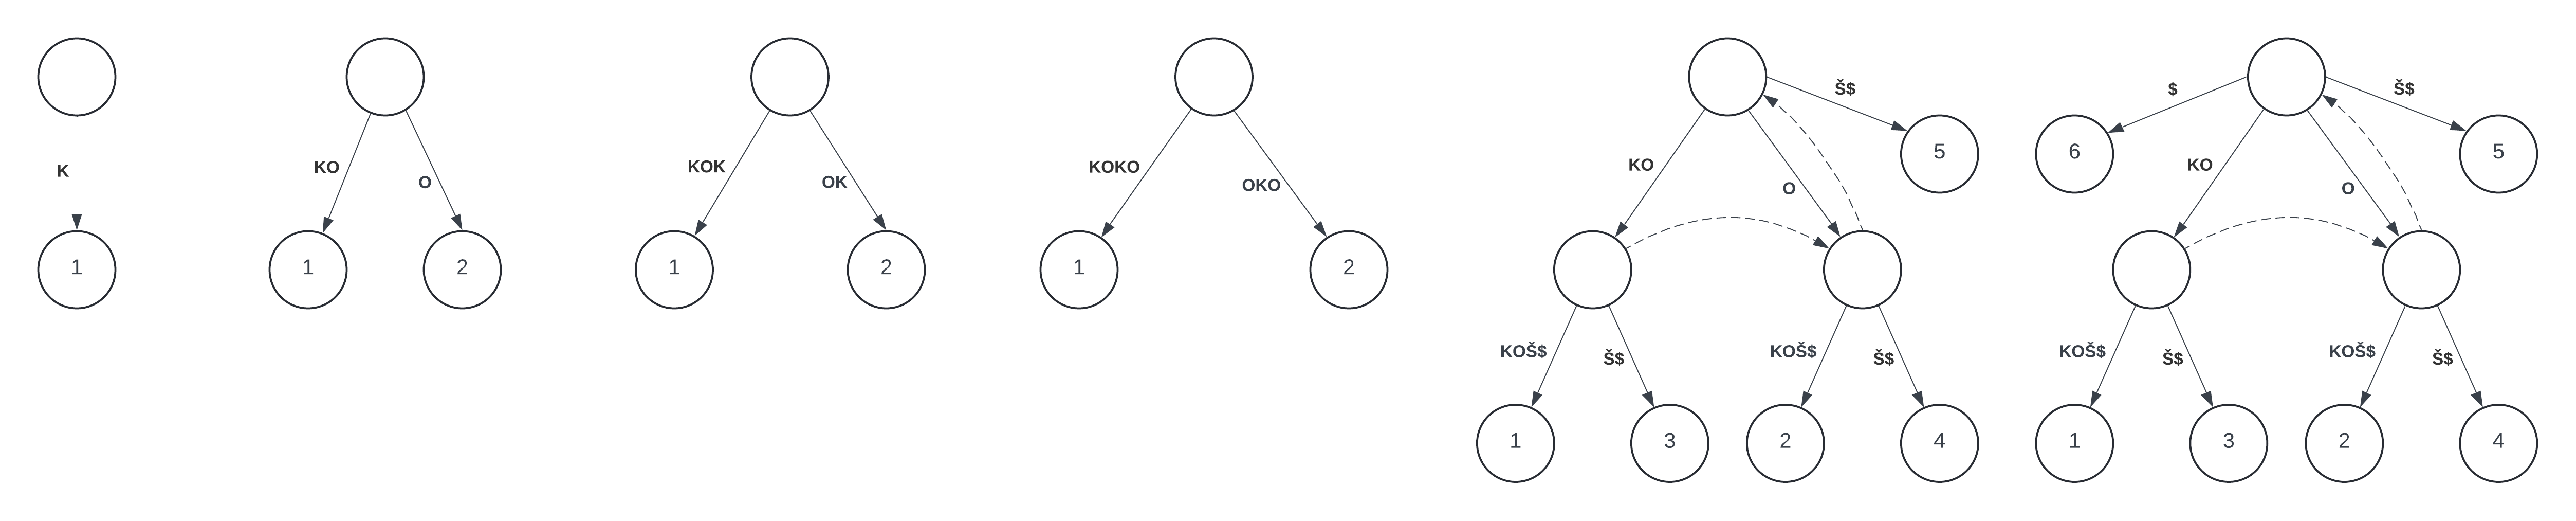
\includegraphics[width=\textwidth]{Slike/KOKOSUkkonen.png}
       \caption{Primer izgradnje priponskega drevesa z uporabo Izboljšane naivne metode za besedo »KOKOŠ$\$$«.} 
        \label{fig:IzbolšanaNaivna}
\end{figure}

Metoda še vedno potrebje beležiti implicitne pripone (pripone, ki so predpone drugim priponam), ampak to beleženje ne vpliva na čas izgradnje priponskega drevesa. Metoda se v vsakem koraku sprehodi iz začetne točke po priponskih povezavah do korena. Postopek izgradnje priponskega drevesa za besedo »KOKOŠ« z izboljšano naivno metodo izgradnje je prikazan na Sliki \ref{fig:IzbolšanaNaivna}. Na sliki je začetna točka označena z zeleno barvo. Ker je v $i$-tem koraku izgradnje največ $i$ eksplicitno definiranih pripon, je tudi število priponskih povezav na poti iz začetne točke do korena po priponskih povezavah enako številu notranjih vozlišč $O(i)$. Torej je čas $i$-tega koraka $O(i)$. Potemtakem ta metoda potrebuje $O(n^2)$ časa za izgradnjo celotnega drevesa. Iz tega sklepa sledi izrek.

\begin{izr}\label{izr:naivnaIzbolsana}
    Izboljšana naivna metoda zgradi priponsko drevo nad besedilom $T$ v času $O(n^2)$.
\end{izr}

%\begin{proof}
%     V $i$-tem koraku izgradnje priponskega drevesa z izboljšano naivno metodo se potrebuje $O(i)$ časa za vstaviti $i$-ti znak v drevo. Ker je besedilo $T$ dolgo $n$ znakov, potem se lahko to zapiše kot
%
%    $$
%        \sum_{i=1}^n i= \dfrac{n(n+1)}{2}=O(n^2).
%    $$
%\end{proof}

Čeprav te izboljšave znižajo čas izgradnje priponskega drevesa na $O(n^2)$, le taka izboljšava ne omogoča izgradnje drevesa v času $O(n)$. Za izgradnjo priponskega drevesa v linearnem času obstajata dva algoritma: McCreightov algoritem \cite{McCreight1976} in Ukkonenov algoritem \cite{Ukkonen1995}. 

\paragraph{McCreightov algoritem:}
McCreightov algoritem ali Algoritem M je prvi algoritem s časovno zahtevnostjo $O(n)$ za izgradnjo drevesa, pri tem pa je tudi prostorska zahtevnost algoritma $O(n)$.
Algoritem deluje, tako da se v $i$-tem koraku v do takrat izgrajeno drevo doda pripona $T[i,n]$. Torej so pripone dodane v drevo v vrstnem redu od najdaljše do najkrajše pripone, za razliko od naivne metode, ki v $i$-tem koraku izgradnje priponskega drevesa doda $i$-ti znak v do takrat izgrajeno priponsko drevo, ki je lahko implicitno. Postopek izgradnje priponskega drevesa za besedo »KOKOŠ« z McCreightvim algoritmom je prikazan na Sliki \ref{fig:McCreight}.

\begin{figure}[htb]
    \begin{subfigure}[t]{0.3\linewidth}
        \subcaption*{}
        \includesvg{Slike/McCreigov/KOKOŠMcCreightKOKOŠ.svg}
        \centering
        \label{fig:McCreigov1}
    \end{subfigure}
    \hspace{0.5cm}
    \begin{subfigure}[t]{0.3\linewidth}
        \subcaption*{}
        \includesvg{Slike/McCreigov/KOKOŠMcCreightOKOŠ.svg}
        \centering
        \label{fig:McCreigov2}
    \end{subfigure}
    \hspace{0.5cm}
    \begin{subfigure}[t]{0.3\linewidth}
        \subcaption*{}
        \includesvg[scale=0.67]{Slike/McCreigov/KOKOŠMcCreightKOŠ.svg}
        \centering
        \label{fig:McCreigov3}
    \end{subfigure}
    
    \begin{subfigure}[t]{0.3\linewidth}
        \subcaption*{}
        \includesvg[scale=0.67]{Slike/McCreigov/KOKOŠMcCreightOŠ.svg}
        \centering
        \label{fig:McCreigov4}
    \end{subfigure}
    \hspace{0.5cm}
    \begin{subfigure}[t]{0.3\linewidth}
        \subcaption*{}
        \includesvg[scale=0.67]{Slike/McCreigov/KOKOŠMcCreightŠ.svg}
        \centering
        \label{fig:McCreigov5}
    \end{subfigure}
    \hspace{0.5cm}
    \begin{subfigure}[t]{0.3\textwidth}
        \subcaption*{}
        \includesvg[scale=0.67]{Slike/McCreigov/KOKOŠMcCreightS.svg}
        \centering
        \label{fig:McCreigov6}
    \end{subfigure}
        \caption{Primer izgradnje priponskega drevesa z uporabo McCreightvega algoritma za besedo »KOKOŠ$\$$«.} 
        \label{fig:McCreight}
\end{figure}

V vsakem koraku je pripona razdeljena na dva dela, in sicer na glavo ter rep. Glava, označena kot $\textit{glava}_i$, je najdaljša predpona $i$-te pripone, ki že obstaja v drevesu. Če take pripone ni v drevesu, je glava pripone prazna. Rep besedila, označen kot $\textit{rep}_i$, pa je definiran kot preostanek pripone, ki ni del glave. Za razliko od glave, rep ne more biti prazen. Ker algoritem temelji na dejstvu, da nobena pripona ni predpona drugi priponi, se mora $n$-ti znak besede razlikovati od ostalih znakov v besedi in se ga označi z znakom »\$«.
Algoritem v vsakem koraku doda krajšo pripono, zato je v repu vedno prisoten vsaj »\$«, saj se bo vedno razlikoval od vsakega znaka, ki je na $(n-i)$-tem mestu poljubne že umeščene pripone \cite{McCreight1976}.

Vsakič, ko se niz $\textit{glava}_i$ ne konča v vozlišču, Algoritem M ustvari novo vozlišče. Ker $\textit{rep}_i$ ni še vsebovan v drevesu, se doda novo list v drevo s povezavo, ki predstavlja niz $\textit{rep}_i$. Repi so dodani v vsakem koraku v konstantnem času, torej algoritem potrebuje zgolj $O(n)$ časa za dodajanje vseh repov.

Glavo $i$-te pripone je možno razdeliti na $\textit{glava}_i = \alpha\beta\gamma$, pri čemer je $\gamma$ lahko prazni podniz. Podniza $\alpha$ in $ \beta$ sta definirana kot dela $\textit{glava}_{i-1} = x\alpha\beta$, pri čemer je $x$ znak $T[i-1]$. Podniz $\alpha$ je prazen niz natanko tedaj, ko je vozlišče, ki predstavlja najdaljšo predpono od $x\alpha$, koren. Če je $\alpha$ prazen, potem je vozlišče $a$, ki je začetna točka iskanja glave, koren. Sicer je vozlišče $a=\textit{sl}(b)$, kjer je $b$ vozlišče, ki predstavlja najdaljšo predpono niza $x\alpha$.

Naslednji korak izgradnje priponskega drevesa je iskanje niza $\beta$ v drevesu. To imenujemo \textit{rescanning}. Po definiciji $\textit{glava}_i$ že obstaja v drevesu, torej obstaja tudi pot iz $a$ v $c$, ki se začne z nizom $\beta$. Iskanje poteka tako, da algoritem primerja dolžino $|\beta|$ z dolžino niza na povezavi iz $a$. Če je $|\beta|$ krajša ali enaka od dolžine niza na povezavi iz $a$, se iskanje prekine. V primeru, da je $|\beta|$ strogo krajša, se ustvari novo vozlišče $d$. Če je $|\beta|$ daljša od dolžine niza na povezavi iz $a$, se izbriše podniz, ki je predstavljen na povezavi, in otrok od $a$ postane novo vozlišče $a$. Postopek se ponovi, dokler $|\beta|$ ni krajša ali enaka od niza, ki ga predstavlja povezava iz $a$. V primeru, da ne obstaja priponska povezava iz vozlišča, ki predstavlja niz $x\alpha\beta$, v vozlišče $d$, se jo ustvari.

Iz vozlišča $d$ se začne iskanje $\gamma$, če le ta ni prazen niz. Ta operacija je imenovana \textit{scanning}. Za razliko od niza $\beta$ dolžina niza $\gamma$ ni znana vnaprej. Algoritem mora zato previti vsak znak, dokler ne najde znaka, ki se razlikuje. Ta znak predstavlja prvi znak v repu. V točki, kjer se znaka razlikujeta, je ustvarjeno novo vozlišče, če ta točka ni že vozlišče. Na to vozlišče se pripne $\textit{rep}_i$.


\begin{izr}
    McCreightov algoritem zgradi priponsko drevo nad besedilom $T$ v času $O(n)$.
\end{izr}

\begin{proof}
    McCreightov algoritem v vsakem koraku naredi tri operacije: operacija vstavljanja repa v drevo, operacijo \textit{scanning} in operacijo \textit{rescanning}. Operaciji  \textit{scanning} in \textit{rescanning} sta v $i$-tem koraku opravljeni nad nizom $\beta_i\gamma_i\textit{rep}_{i}$. 
    
    Za vstaviti rep v drevo algoritem potrebuje $O(1)$ časa. V drevo je potrebno vstaviti $n$ pripon, torej je potreben čas za vstaviti vse repe v drevo $T_{\textit{rep}}=O(n)$.

    Operacija \textit{scanning} potrebuje v vsakem koraku $|glave_i|-|glave_{i-1}|+1=|\gamma_i|$ časa. Torej po vseh korakih operacija \textit{scanning}  potrebuje $T_{\textit{scan}}=\sum_{i=1}^n |glave_i|-|glave_{i-1}|+1= n + |glava_n|-|glava_0|=O(n)$ časa.

    V $i$-tem koraku operacija \textit{rescanning} obišče $n_i$ vozlišč. Pri tem se opazi, da v naslednjem koraku ta vozlišča ne bodo obiskana. Iz tega sledi:  $|\beta_{i+1}\gamma_{i+1}\textit{rep}_{i+1}|\le|\beta_i\gamma_i\textit{rep}_{i}|-n_i$, pričemer je $|\beta_n\gamma_n\textit{rep}_{n}|=|\textit{rep}_{n}|=1$. Torej velja tudi:    
    \begin{equation*} 
        \begin{split}
        |\beta_n\gamma_n\textit{rep}_{n}|=|\textit{rep}_{n}|&\le|\beta_1\gamma_1\textit{rep}_{1}|- \sum_{i=1}^n n_i,\\
        1&\le n- \sum_{i=1}^n n_i,\\
        n&\ge 1+ \sum_{i=1}^n n_i.
        \end{split}
    \end{equation*}
    
    Iz tega sledi, da operacija \textit{rescanning} skozi celotno izgradnjo obišče največ $n$ vozlišč, zato potrebuje $T_{\textit{rescan}}=O(n)$ časa skozi celotno izgradnjo.
    
    Torej je potrebni čas za izgradnjo priponskega drevesa vsota časov potrebnih za posamezno operacijo: 
    $$T_{\textit{izgradnja}}=T_{\textit{rep}}+T_{\textit{rescan}}+T_{\textit{scan}}=O(n)+O(n)+O(n)=O(n).$$
\end{proof}

Čeprav McCreightov algoritem zgradi priponsko drevo v času in prostoru $O(n)$, algoritem predpostavi, da je beseda $T$ vnaprej poznana. Pri tem se pojavi vprašanje, ali je mogoče izgraditi priponsko drevo, ne da bi vnaprej poznali začetno besedo. Metoda, ki ne potrebuje celotne besede vnaprej, je Ukkonenov algoritem, ki priponsko drevo zgradi sprotno (angl. \textit{on-line}), kot ga je izgradila tudi naivna metoda, ter potrebuje $O(n)$ časa in prostora.

\paragraph{Ukkonenov algoritem:}
Ukkonenov algoritem deluje na podoben način kot prej predstavljena naivna metoda, saj dodaja v drevo črko po črko. Torej algoritem v $i$-tem koraku izgradi priponsko drevo, ki je lahko implicitno priponsko drevo, in predstavlja besedilo $T[1,i]$. Primer  izgradnje drevesa z Ukkonenovim algoritmom, je prikazan na Sliki \ref{fig:Ukkonen}. Algoritem v $i$-tem koraku doda v drevo črko $x$. Naj bo $\alpha$ niz, ki z $x$ tvori niz $T[a,i]=\alpha x$, pri čemer je $1\le a <i $ in posledično je $\alpha$ lahko prazen niz. Znak $x$ je lahko dodan v drevo na tri načine:

\begin{enumerate}
    \item Če se niz $\alpha$ konča v listu, potem se zadnja povezava, ki je del niza $\alpha$, podaljša  za znak $x$. Torej enkrat, ko je list zgrajen, ne more postati notranje vozlišče. Način je prikazan na Sliki \ref{fig:aUkkonen1}.
    \item Če pa se niz $\alpha$ ne konča v listu, potem se konča bodisi v vozlišču $v$, bodisi na povezavi med vozliščema, recimo $v_1$ in $v_2$. V tem primeru se lahko znak $x$ doda na dva načina:
    \begin{enumerate}
        \item \label{enum:dodajanje2} Če se nobena pot ne nadaljujeki z znakom $x$, se ustvari nov list $l$, na katerega kaže poveznava z oznako $x$. Če se niz $\alpha$ konča v vozlišču $v$, potem $l$ postane otrok vozlišča $v$. Če pa se $\alpha$ konča sredini niza na povezavi med vozliščema $v_1$ in $v_2$, se ustvari novo vozlišče $v'$. Povezava, ki kaže iz vozlišča $v_1$ na vozlišče $v'$, predstavlja niz, ki se je ujeml z $\alpha$. Iz novega vozlišča kažeta dve povezavi: prva povezava kaže na list $l$, druga povezava pa kaže na vozlišče $v_2$, ki predstavlja preostanek niza, ki ga je predstavljala predhodnja povezava. Način je prikazan na Sliki \ref{fig:aUkkonen2}.
        \item Če pa obstaja taka pot, ki se nadaljuje po nizu $\alpha$ z znakom $x$, se ne stori ničesar, saj je drevo že v implicitni obliki. Način je prikazan na Sliki \ref{fig:aUkkonen3}.
    \end{enumerate}    
\end{enumerate}

\begin{figure}[htb]
    \begin{subfigure}[t]{0.3\linewidth}
        
        \includesvg[scale=0.67]{Slike/Abs/UkkonenIzgradnjaAbstraknoNači1.svg}
        \centering
        \subcaption{}
        \label{fig:aUkkonen1}
    \end{subfigure}
    \hspace{0.5cm}
    \begin{subfigure}[t]{0.3\linewidth}
        
        \includesvg[scale=0.67]{Slike/Abs/UkkonenIzgradnjaAbstraknoNači2.svg}
        \centering
        \subcaption{}
        \label{fig:aUkkonen2}
    \end{subfigure}
    \hspace{0.5cm}
    \begin{subfigure}[t]{0.3\linewidth}
        \includesvg[scale=0.67]{Slike/Abs/UkkonenIzgradnjaAbstraknoNači3.svg}
        \subcaption{}
        \centering
        \label{fig:aUkkonen3}
    \end{subfigure}    
        %   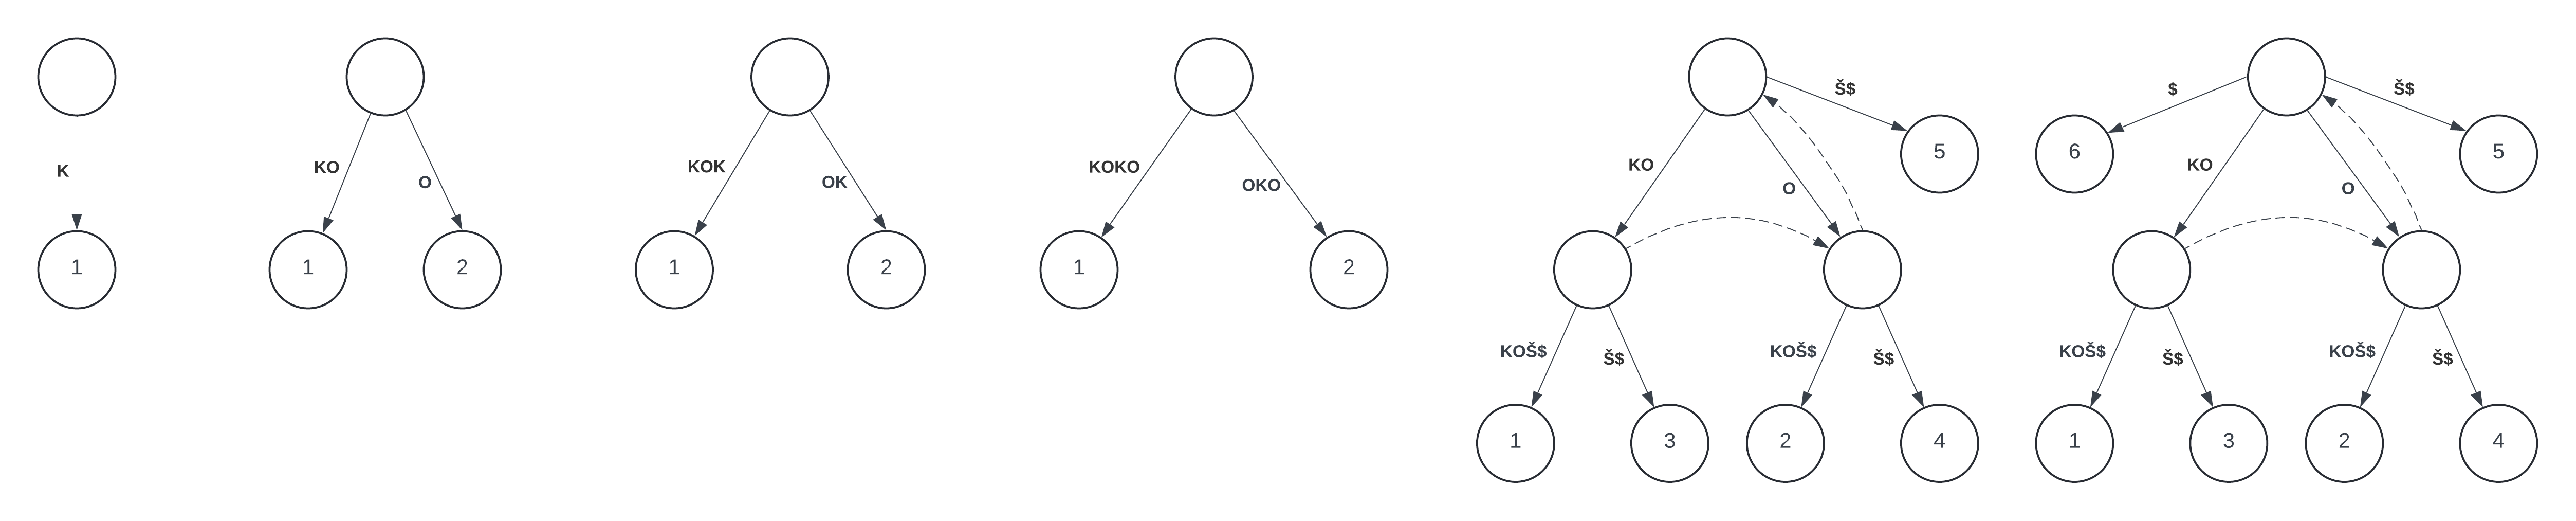
\includegraphics[width=\textwidth]{Slike/KOKOSUkkonen.png}
           \caption{Načini dodajanja novih znakov v priponsko drevo.} 
            \label{fig:absUkkonen}
    \end{figure}



Iz načina dodajanja novih znakov v priponsko drevo, ki ga uporablja algoritem, se opazi, da se število vozlišč v drevesu spremeni samo z drugim načinom dodajanja (\ref{enum:dodajanje2}). Da bo algoritem učinkovit, se hraniti začetek, ki ga imenujemo začetna točka, in konec, ki ga imenujemo končna točka (angl. \textit{end point}), rezčlembe ter dodajanja novih vozlišč v drevesu v trenutnem koraku. Na Sliki \ref{fig:Ukkonen} je z rdečo označeno vozlišče, ki se nahaja pred končno točko, ter z zeleno je označeno vozlišče, ki pa se nahaja pred začetno točko. Vse točke, v katerih se bo v tem koraku zgodila razčlemba, imenujemo aktivne točke (angl. \textit{active point}). Začetna točka je prva aktivna točka, končna točka pa je zadnja aktivna točka v trenutnem koraku dodajanja. Premik po aktivnih točkah med začetno točko in končno točko poteka po priponskih povezavah. Pri tem pa algoritem v vsakem koraku poti izračuna, ali je že prišel v končno točko. Za to je potrebno hraniti zgolj trenutno aktivno točko ter zastavico, ki hrani vrednost ali je ta točka tudi končna točka. Pri tem velja tudi, da končna točka v koraku $i-1$ postane aktivna točka v koraku $i$, saj se prva nova razčlemba v koraku $i$ lahko zgodio zgolj v točki, kjer se je končala razčlemba v koraku $i-1$ in to je končna točka koraka $i-1$. 

\begin{figure}[htb]
    \begin{subfigure}[t]{0.3\linewidth}
        \subcaption*{}
        \includesvg{Slike/Ukkonen/KOKOŠUkkonenK.svg}
        \centering
        \label{fig:Ukkonen1}
    \end{subfigure}
    \hspace{0.5cm}
    \begin{subfigure}[t]{0.3\linewidth}
        \subcaption*{}
        \includesvg{Slike/Ukkonen/KOKOŠUkkonenOKOŠ.svg}
        \centering
        \label{fig:Ukkonen2}
    \end{subfigure}
    \hspace{0.5cm}
    \begin{subfigure}[t]{0.3\linewidth}
        \subcaption*{}
        \includesvg{Slike/Ukkonen/KOKOŠUkkonenKOŠ.svg}
        \centering
        \label{fig:Ukkonen3}
    \end{subfigure}
    
    \begin{subfigure}[t]{0.3\linewidth}
        \subcaption*{}
        \includesvg{Slike/Ukkonen/KOKOŠUkkonenOŠ.svg}
        \centering
        \label{fig:Ukkonen4}
    \end{subfigure}
    \hspace{0.5cm}
    \begin{subfigure}[t]{0.3\linewidth}
        \subcaption*{}
        \includesvg[scale=0.67]{Slike/Ukkonen/KOKOŠUkkonenŠ.svg}
        \centering
        \label{fig:Ukkonen5}
    \end{subfigure}
    \hspace{0.5cm}
    \begin{subfigure}[t]{0.3\textwidth}
        \subcaption*{}
        \includesvg[scale=0.67]{Slike/Ukkonen/KOKOŠUkkonenS.svg}
        \centering
        \label{fig:Ukkonen6}
    \end{subfigure}

    %   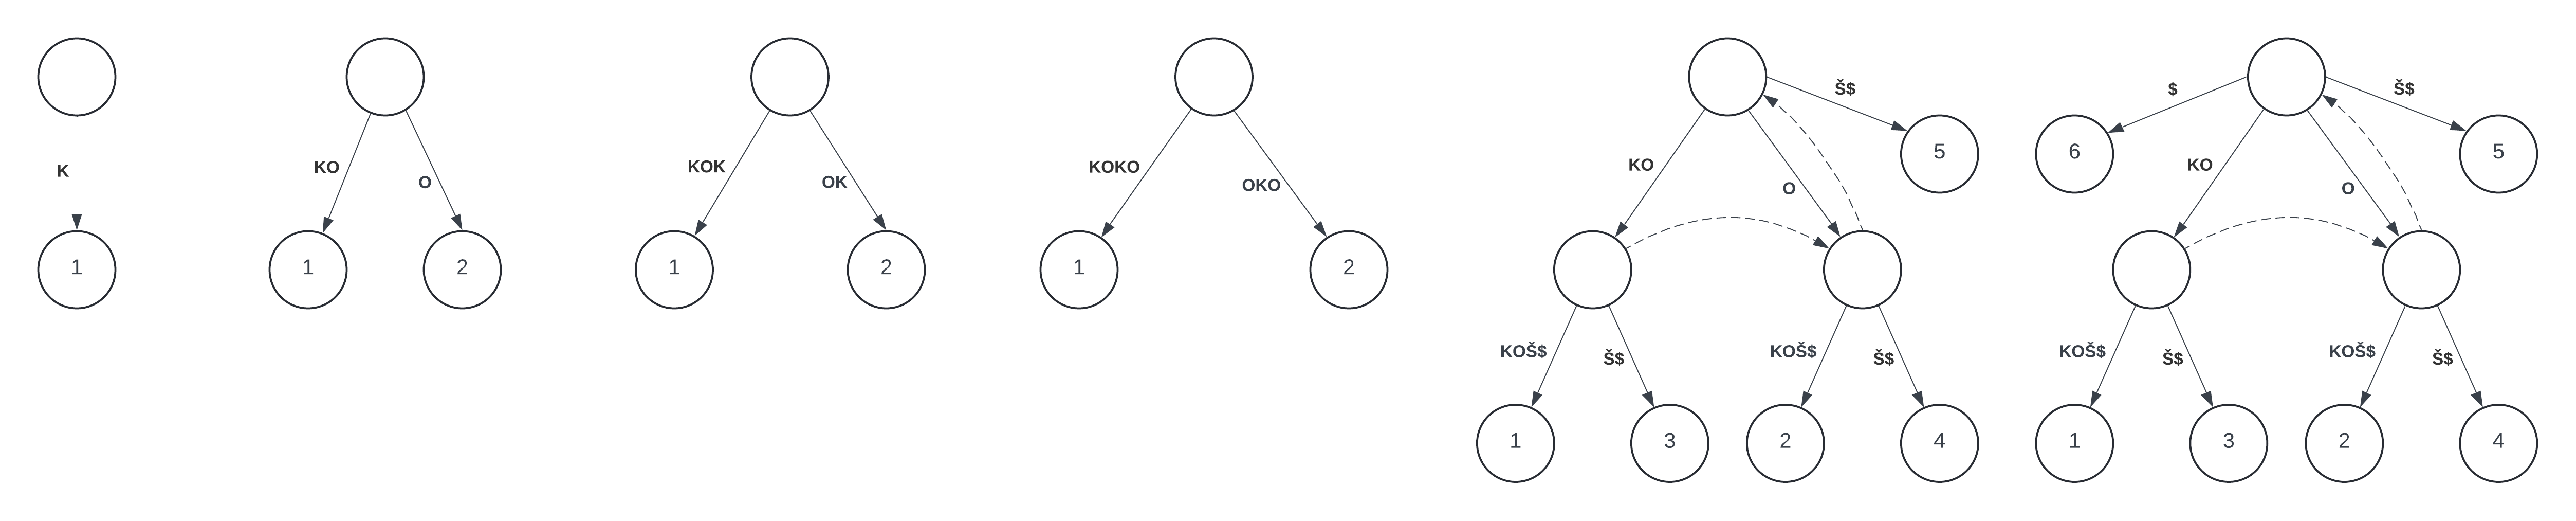
\includegraphics[width=\textwidth]{Slike/KOKOSUkkonen.png}
       \caption{Primer izgradnje priponskega drevesa z uporabo Ukkonenovaga algoritma za besedo »KOKOŠ$\$$«.} 
        \label{fig:Ukkonen}
\end{figure}

Vsako aktivno točko lahko predstavimo kot referenčni par $(s,\alpha)$, pri čemer je $s$ vozlišče pred aktivno točko in $\alpha$ je niz iz vozlišča $s$ do aktivne točke. Za lažje shranjevanje niza $\alpha$ je le ta shranjen kot par indeksov $(k,p)$, pri čemer je $\alpha=T[k,p]$. Ker je lahko aktivna točka predstavljena z različnimi referenčnimi pari $(s,(k,p))$, se zato lahko za $s$ izbere najglobje vizlišče pred aktivno točko. Takšen par je enoličen in ga imenujemo kanonična oblika referečnega para. Med vsemi referenčnimi pari za dano aktivno točko velja, da je pri paru, ki je v kanonični obliki, niz $\alpha=T[k,p]$ najkrajši. Na Sliki \ref{fig:Ukkonen} v četrtem koraku izgradnje, ki ga predstavlja prvo drevo v spodnji vrstici, je začetna aktivna točka predstavljena kot $(\textit{koren},(1,3))$, v naslednjem koraku pa je začetna aktivna točka v $(\textit{koren},(1,4))$, ki se bo razcepila in bo postala novo vozlišče. Ta ista točka je lahko po koncu izgradnje še vedno predstavljena z referenčnim parom $(\textit{koren},(1,4))$, ki pa ni v kanonični obliki. Kanonična oblika te točke je $(a,(4,4))$, pri čemer je vozlišče $a$ otrok \textit{koren}-a, na katerega kaže povezava z nizom »KO«.

\begin{algorithm}[htb]

    \Vhod{Besedilo $T$, dolžine $n$}
    \Izhod{Priponsko drevo}
    \caption{Ukkonenov algoritem za izgradnjo priponskega drevesa}\label{alg:ukkonen}
    {
        {Ustvari vozlišče \textit{koren}}
        
        {$s$<- \textit{koren}, k<-1}
        
        \Za{$i = 1, \ldots, n$}{\label{vrstica:zankaDodajanje}
    
    
            {\textit{sVoz}<-\textit{NIL}}
            
            {$(\textit{KončnaTočka},v)$<-\texttt{razdeliTestiraj}($s,k,i-1,T[i]$)}
            
            \Dokler{ni \textit{KončnaTočka}}{\label{vrstica:zankaKončnatočka}
    
                {ustvari list $v'$ na katerega kaže točka $v$}
    
                \Ce{$\textit{sVoz} \ne \textit{NIL}$}
                    {Ustvari priponsko povezavo iz \textit{sVoz} v $v$}
    
                {\textit{sVoz}<-$v$}
                 
                {$(s,k)$<-\texttt{kanoničnaOblika}($sv(s),k,i-1$)}
                
                {$(\textit{KončnaTočka},v)$<-\texttt{razdeliTestiraj}($s,k,i-1,T[i]$)}
            }
            
            \Ce{$\textit{sVoz} \ne \textit{NIL}$}
                    {Ustvari priponsko povezavo iz \textit{sVoz} v $s$}
                    
            {$(s,k)$<-\texttt{kanoničnaOblika}($s,k,i$)\label{vrstica:povečavaBeta}}
            
        }
        
    }
\end{algorithm}

Ukkonenov algoritem za izgradnjo priponskega drevesa, ki je predstavljen v \cite{Ukkonen1995}, izgradi priponsko drevo s psevdokodo, ki je prikazana v Algoritmu \ref{alg:ukkonen}.
V algoritmu $s$ predstavlja najglobje vozlišče pred aktivno točko ter $k$ predstavlja indeks začetne črke niza iz vozlišča $s$ proti aktivni točki v besedilu $T$. Številka $i$ predstavlja indeks črke v $T$, ki je dodana v drevo. Vozlišče $s$ ter par števil $(k,i-1)$ predstavljajo aktivno točko v trenutnem koraku. Zastavica \textit{KončnaTočka} ima vrednost \textit{true}, če je trenutna aktivna točka tudi končna točka, sicer ima vrednost \textit{false}. Vozlišče $v$ predstavlja vozlišče, v katerega bo pripet nov list $v'$. Povezava do lista $v'$ bo predstavljala črko $T[i]$. Vozlišče \textit{sVoz} pa predstavlja vozlišče, na katerga je bil nazadnje pripet list v $i$-tem koraku. Vozlišče \textit{sVoz} je \textit{NIL} zgolj v prvem dodajanju novega lista v vsakem koraku.


Algoritem \ref{alg:ukkonen} uporabi dve pomožni funkciji. Prva uporabljena pomožna funkcija je \texttt{kanoničnaOblika}, ki pretvori trenutno aktivno točko priponskega drevesa v kanonično obliko. Funkcija prejme kot vhod vozlišče $s$ ter niz, predstavljen kot položaj začetka $k$ in konca $p$ podniza do aktivne točke v nizu $T$. Funkcija se sprehodi po drevesu dokler ne doseže najnižjega vozlišča pred aktivno točko. S tem korakom je omogočena učinkovitejša uporaba funkcije \texttt{razdeliTestiraj}.

Funkcija \texttt{razdeliTestiraj} prejme kot vhod znak $t$, ki se želi vstaviti v priponsko drevo, ter trenutno aktivno točko, ki je podana kot referenčni par $(s,(k,p))$ v kanonični obliki. Funkcija preveri ali se niza $T[k,p+1]$ in $T[k,p]\cdot t$ ujemata. Če se niza ujemata, potem je trenutna aktivna točka tudi končna točka, zato funkcija ne stori ničesar in vrne $(\textit{true},s)$. Sicer pa funkcija razdeli povezavo in aktivna točka postane novo vozlišče $v$, če že ne obstaja vozlišče $v$, nato pa vrne $(\textit{false},v)$. 


\begin{izr} \label{izr:ukkonen}
    Ukkonenov algoritem zgradi priponsko drevo nad besedilom $T$ v času $O(n)$.
\end{izr}


\begin{proof}

Dokaz je razdeljen na dva dela: v prvem delu bomo dokazali, da se zanka, ki se začne v vrstici \ref{vrstica:zankaKončnatočka}, skozi celotno izvajanje algoritma izvede $O(n)$-krat, drugi del pa se bo osredotočil na časovno zahtevnost funkcije \texttt{kanoničnaOblika}. 

Časovna zahtevnost funkcije \texttt{razdeliTestiraj} je $O(1)$, saj funkcija prever ali če je trenutna aktivna točka tudi končna točka in posledično če ni končna točka jo spremeni v notranje vozlišče. Ker je aktivna točka podana v kanonični obliki, ni potrenbnih odvečnih sprehodov po drevesu, ki bipovečali časovno zahtevnost.

Zanka v $i$-tem koraku izgradnje, dodaja nove povezave na poti iz končne točke $kt_{i-1}$ koraka $i-1$, do končne točke $kt_i$ koraka $i$, katera ni še obiskana. Natančno število obiskanih vozlišč na poti je $D(kt_{i-1})-D(kt_i)+2$, iz česar sledi, da se s pomočjo seštevalne amortizacije v $n$-tih korakih zanka izvede


$$
    \sum_{i=1}^n \left(D(kt_{i-1})-D(kt_i)+2\right)=D(kt_0)-D(kt_n)+2n=O(n).
$$

Pri tem je potrebno še dokazati, da tudi sprehod v funkciji \texttt{kanoničnaOblika} obišče $O(n)$ vozlišč skozi celotno izgradnjo priponskega drevesa. Funkcija ob vsakem klicu pogleda največ $p-k$ vozlišč, kar je dolžina niza $\beta=T[k,p]$. Pri tem pa se niz $\beta$ z vsakim obiskanim vozliščem skrajša, saj se poveča število $k$. Niz $\beta$ pa se lahko poveča zgolj v \ref{vrstica:povečavaBeta} vrstici Algoritma \ref{alg:ukkonen}. Ker se niz $\beta$ poveča $n$-krat skozi celotno izgradnjo, potemtakem se tudi niz $\beta$ lahko zmanjša največ $n$-krat skozi celotno izgradnjo. Torej funkcija \texttt{kanoničnaOblika} obišče največ $n$ vozlišč v celotni izgradnji priponskega drevesa.


Zanka v vrstici \ref{vrstica:zankaDodajanje} Algoritma \ref{alg:ukkonen} se izvede $n$-krat, medtem ko se zanka v vrstici \ref{vrstica:zankaKončnatočka} in funkcija \texttt{kanoničnaOblika} vsaka izvede v $O(n)$ časa skozi celotno izgradnjo priponskega drevesa, iz česar sledi, da tudi izgradnja priponskega drevesa potrebuje $O(n)$ časa, da se izvrši.
  
\end{proof}

\paragraph{Zaključek:}
Tako McCreight algoritem \cite{McCreight1976} kot tudi  Ukkonenov algoritem \cite{Ukkonen1995} zgradita priponsko drevo v času $O(n)$. Oba algoritma izdelata priponsko drevo, ki ima enake priponske povezave med vozlišči, pri tem pa se zalikujeta v umesnih drevesih. Za primerjavo umesnih dreves se lahko vzame Sliko \ref{fig:McCreight} in Sliko \ref{fig:Ukkonen}, na katerih sta prikazani izgradnji priponskih dreves z obema algoritma za besedo »KOKOŠ\$«. V McCreightovem algoritmu vmesno drevo v $i$-tem koraku predstavlja $i$ najdaljših pripon besedila. Pri čemer pa v Ukkonenovem algoritmu vmesno drevo v $i$-tem koraku predstavlja priponsko drevo besedila $T[1,i]$, ki je lahko bodisi implicitno bodisi eksplicitno predstavljeno, kar je posledica sprotne izgradnje priponskega drevesa.

Poleg linearne časovne zahtevnosti za izgradnjo priponskega drevesa, oba algoritma potrebujeta $O(n)$ prostora za hrambo in gradnjo priponskega drevesa, saj ima vsako drevo $n$ listov in največ $n-1$ notranjih vozlišč. Vsako vozlišče ima $O(|\Sigma|)$ referenc, pri čemer je $\Sigma$ abeceda vseh znakov uporabljenih v besedilu. Za daljša besedila je to lahko problem, saj velikost celotnega priponskega drevesa lahko presega velikost delovnega pomnilnika.

V nadaljevanju bo uporabljen Ukkonenov algoritem za izgradnjo priponskih dreves, ki bodo uporabljena pri empirični analizi v Poglavju \ref{sec:primerjava}, kjer bo tudi izmerjen vpliv pomanjkanja notranjega pomnilnika ter posledična uporaba zunanjega pomnilnika (\verb|Swap| razdelek na zunanjem spominu) namesto notranjega pomnilnika.